% -*- mode: LaTeX; coding: utf-8; -*-

\chapter{Tutkimusasetelma}

Edellisissä luvuissa on esitetty pieni osa niistä hyökkäyksistä, joita vastaan verkot ja web-palvelut joutuvat nykyisin suojautumaan. Niiden suuresta määrästä johtuen on ilmiselvää, että täysin 
turvallista ympäristöä on mahdoton rakentaa. Yleensä tämä ei ole edes tietoturvasuunnittelun lähtökohtana, vaan tärkeämpää on löytää tasapaino palvelun saatavuuden, ja käytettyjen tietoturvaratkaisuiden 
välillä. Liian raskaat menetelmät aiheuttavat ylimääräistä viivettä palvelun tai verkon saatavuuteen, ja liian kevyet ratkaisut jättävät ne avoimiksi yleisimmille hyökkäyksille. 

\section{Lähtökohta}

Tämän Pro gradu-tutkielman tavoitteena on pyrkiä tunnistamaan web-palveluihin kohdistuvia poikkeavuuksia analysoimalla palvelimien tallentamaa tapahtumalokia. Analysoitava data on Apache-palvelimien 
tuottamaa lokia, joka sisältää web-palveluille kohdistuvia HTTP-pyyntöjä. Loki noudattaa CLF-formaattia (Common Log Format), jota web-palvelimet käyttävät lokitiedon tallentamiseen. Se on standardoitu 
formaatti, jossa jokaisella rivillä on tietynlainen syntaksi. Kuvassa \ref{CLF} on esitetty yhdestä HTTP-pyynnöstä syntyvä lokirivi. 

Analysoitava loki on saatu Ixonos Oy:ltä, joka tarjoaa muiden palveluiden ohella hosting-palveluita suuryrityksille. Kyseinen loki on peräisin tuotannosta jo poistetuilta palvelimilta, jotka ovat olleet
vastuussa muutaman suuren palvelukokonaisuuden pyörittämisestä. Lokia on yhteensä ?? gigatavua, ja se sisältää yli ?? miljardia sivupyyntöä, joista ??? on tullut uniikista IP-osoitteesta. Loki on kerätty
noin 10 kuukauden ajanjaksolta.

\vspace{3mm}

\begin{figure}[ht]
\centering
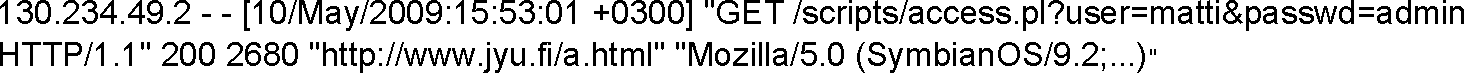
\includegraphics[width=15cm]{pics/logi.pdf}
\caption{Esimerkki web-palvelimen tuottamasta logista}
\label{CLF}
\end{figure}

Web-palvelimien tuottama loki sisältää paljon tietoa mm. palveluiden käyttöasteista, ja niihin kohdistuvista kuormista. Niitä analysoimalla voidaan myös tunnistaa mahdollisia hyökkäysyrityksiä, sekä
hyökkäyksen jo tapahduttua tutkia siihen johtaneita vaiheita. Pienillä sivustoilla lokin läpikäyminen jälkikäteen käsin on vielä mahdollista, mutta puhuttaessa palveluista, joilla on miljoonia käyttäjiä 
kuukaudessa, ei tämä ole enää mahdollista. Tästä syystä lokien analysoiminen tulee automatisoida. Tämä taas johtaa siihen, että järjestelmän tulisi pystyä tunnistamaan miljoonien kyselyiden joukosta
ne, jotka ovat syntyneet hyökkäyksen johdosta. Yksi mahdollisuus on käyttää sääntöpohjaista ratkaisua, mutta aikaisemmin esitetyistä syistä johtuen, ei tämä tarjoa aina riittävää tunnistuskykyä. Tästä 
syystä olemme päätyneet käyttämään anomalioiden tunnistamismenetelmää, jossa järjestelmälle opetetaan normaali käyttäytyminen. Tämän jälkeen haluttu data verrataan opetettuun malliin, jolloin poikkeava
liikenne voidaan tunnistaa.

Tietoturvan kannalta kiinnostavin osa logista on GET-parametrin jälkeinen osa, jossa kuljetetaan varsinainen HTTP-pyyntö. Tämä sisältää niin staattiset sivunlatauspyynnöt, kuin myös palvelimelle 
välitettävät parametriarvot. Tällaisia voivat olla esimerkiksi kirjautumisessa käytetyt tiedot, ja tietokannalle välitetyt kyselyt. Staattiset sivunlatauspyynnöt ja parametreja sisältävät pyynnöt erottaa
resurssipolun jälkeisestä kysymysmerkistä. Kysymysmerkin jälkeinen kyselyosuus koostuu avain-arvo-pareista, joista ensimmäinen on kutsuttu parametri, ja jälkimmäinen tämän arvo (kuva \ref{CLF2}). Riippuen
palvelun toteutuksesta näitä voi olla useampia peräkkäin \&-merkillä erotettuna.

\begin{figure}[ht]
\centering
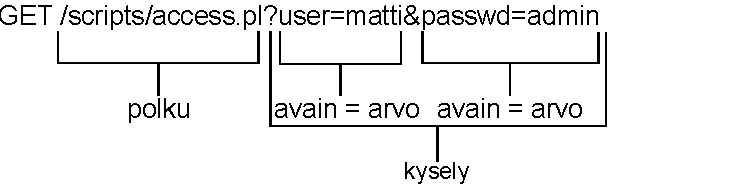
\includegraphics[width=13cm]{pics/logi2.pdf}
\caption{HTTP-kyselyn GET-osa}
\label{CLF2}
\end{figure}

\section{Käytettyjen menetelmien yleinen kuvaus}

Ongelmia lokin analysoimisessa aiheuttaa sen suuri määrä ja käytössä olevat parametrit. Näistä osa on luokka-asteikollisia ja osa taas numeroasteikollisia, joten tietynlaisten toimintamallien etsiminen näistä
ei suoraan onnistu. Parametrien suuri määrä aiheuttaa myös laskennallisia ongelmia, joten niiden määrää tulee pystyä jotenkin vähentämään säilyttäen kuitenkin mahdollisimman tarkkaan alkuperäisten muuttujien 
piirteet. Seuraavaksi esitetään yleisellä tasolla käytetyt tekniikat, ja sitä seuraa näiden tarkempi matemaattinen kuvaus.

Anomalioiden tunnistamiseen käyttämämme järjestelmä pohjautuu diffuusiokuvausten ja diffuusioetäisyyksien käyttöön, jotka tarjoavat tehokkaan tavan löytää merkittäviä geometrisia rakenteita datasta. Näiden
käyttämistä moniulotteisen datan esittämisessä on esitelty \cite{diff} \cite{diff2}. Menetelmien tehokkuus perustuu siihen, että diffuusiokuvausten avulla pystytään vähentämään analysoitavan datan dimensioita
säilyttäen kuitenkin sen rakenne. Periaatteessa dimensioiden vähentäminen tarkoittaa sitä, että datajoukko esitetään toisella datajoukolla, jonka dimensio on pienempi. Tällöin sen analysoiminen ja esittäminen
graafisesti on helpompaa.

Dimensioiden vähentäminen tapahtuu laskemalla diffuusioetäisyydet eli keskimääräiset arvot kaikista kahden pisteen välisistä poluista ts. todennäköisyydet kulkea satunnaiskululla pisteestä toiseen kiinteällä
askelmäärällä. Tällä tavoin lasketut etäisyydet ovat vähemmän herkkiä topologiamuutoksille, joita dimensioiden vähennys aiheuttaa. Diffuusioetäisyydet saadaan myös nopeasti laskettua vektorien ominaisarvoista, 
joten menetelmää voidaan käyttää reaaliajassa riittävän pienellä viiveellä. 

Analysoitavan datan luonteesta johtuen pelkkä dimensioiden vähentäminen ei tuo esille poikkeavuuksia, vaan tätä varten tarvitaan parametreja, jotka kuvaavat HTTP-pyynnön sisältöä tarkemmin. Suurimmasta osasta kyselyn
sisältämistä parametreista kuten IP-osoitteesta, ajasta tai käytetystä selaimesta tämä ei käy ilmi. Toki näistä voidaan tunnistaa esimerkiksi hyökkäykset, joissa yritetään kuluttaa palvelimen resurssit loppuun
hakemalla samaa tiedostoa yhä uudestaan tai pommittamalla uusia yhteysyrityksiä. Web-palveluihin kohdistuvat hyökkäykset ovat kuitenkin usein paljon hienovaraisempia. Parhaiten näitä voidaan yrittää tunnistaa
tutkimalla tarkemmin GET-parametrin jälkeistä osaa, josta käy ilmi parametrit, joita hyökkääjä välittää palvelimelle. 

Tietoturvahyökkäyksissä hyökkääjä pyrkii aina ohittamaan jollakin tavalla asetetut suojaukset. Usein tämä tarkoittaa sitä, että palvelimelle välitetyt pyynnöt muodostuvat pitkistä merkkijonoista, ja niissä käytetyt
merkit poikkeavat normaalisti käytetyistä merkeistä. Useiden peräkkäisten avain-arvo parien määrä myös saattaa kasvaa reilusti normaalia suuremmaksi. Näiden tunnistamista varten käytämme analyysissa n-gram analyysiksi
kutsuttua menetelmää, jossa selvitetään käytettyjen merkkien normaali jakauma ja järjestys. Analyysi voidaan tehdä esimerkiksi koko kyselylle, avain-arvo pareille tai pelkästään tietylle resurssille. 

N-gram analyysin tuottamat matriisit ovat tässä tapauksessa niin moniulotteisia, että dimensioiden määrä tulee pystyä jollakin tavalla vähentämään. Tämä onnistuu satunnaisprojektion avulla, joka on dimensioiden
vähentämiseen tarkoitettu tekniikka. Satunnaisprojektiossa moniulotteinen data heijastetaan pienempi ulotteiseen aliavaruuteen käyttäen satunnaisesti luotua matriisia. Näin syntynyt uusi matriisi on laskennallisesti
tehokas, ja se on riittävän tarkka menetelmä dimensioiden vähentämisessä. 

\subsection{Diffuusiokuvaus}

\subsection{n-gram analyysi}

\subsection{Satunnaisprojektio}



%- mistä lähtökohdista lähdetään tutkimaan eli mitä materiaalia on käytössä
%- mitä voidaan etsiä käytössä olevasta materiaalista
%- mitä menetelmiä käytetään (n-gram, diffuusiokuvaus, satunnaisprojektio)
%- korkeamman tason selitys mitä tehdään
%- menetelmien tarkka kuvaus
